\scanpage{94}

\textcircled{5.} \uline{Remarkable classes of operators in Hilbert space}

We begin by giving an {\color{red}\uline{\color{black}exposition}} of Schatten's theory, \deleted{\unsure{which is|which we}} in a simplified form made possible by the \deleted{\unsure{lemma}}\inserted{\unsure{minimum|minimax} method} of Weyl, and by {\color{red}\uline{\color{black}adding to it}} a few \unsure{small|minor} supplements.

{\reversemarginpar\margin{{\color{red}?}}}

\deleted{\unsure{Definition}} Let us recall the

{\reversemarginpar\margin{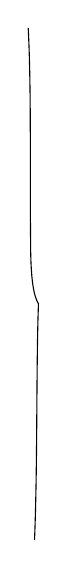
\begin{tikzpicture}[baseline=(current bounding box.north)]\draw[line width=.4pt] (0,0) .. controls (.04,-.8) and (.02,-1.7) .. (.03,-2.7) .. controls (.03,-3.2) and (.07,-3.4) .. (.13,-3.5) .. controls (.10,-4.3) and (.12,-5.5) .. (.08,-6.5);\end{tikzpicture}}}
\uline{Definition 1} \deleted{Let} A norm $N$ on $R^n$ is called a \uline{Schatten norm} if it is symmetric, satisfies

\deleted{\unsure{to|2|3}}

\[
\begin{array}{@{}l@{\qquad}l@{}}
(1)&\displaystyle N(x_1,\mathord{-}x_n)=N(|x_1|,\mathord{-}|x_n|)
\end{array}
\]

\deleted{and if it} \unsure{if|2.} it is increasing \deleted{\unsure{on the set}} on the set of $x_i\geq 0$, and \deleted{\unsure{is satisf}} is normalized by $N(1,0,\mathord{-}0)=1$

A norm $N$ on $R^{(\underline N)}$ \deleted{$\unsure{R}\underline N$ \unsure{set|space of}} (\unsure{space|ring} of infinite sequences \deleted{\unsure{finite}} zero except for a finite number of terms) is called a Schatten norm, if \inserted{for every integer $n>0$,} it induces \deleted{on} of on $R^n$ a Schatten norm

($R^n$ will here be identified \deleted{\unsure{with the space of sequences}}\inserted{with the subspace} of $R^{(\underline N)}$ consisting of the sequences zero from index $n+1$ onwards). Note that a Schatten norm on $R^n$ induces on $R^m$ ($m\leq n$) a Schatten norm. \deleted{\unsure{All this theory yields that|It is immediate that}}\inserted{Examples of norms of} Schatten\,:

\deleted{\unsure{Suppose|the map}}

\[
\deleted{N_p(\{x_i\})\unsure{=}\left(\sum |x_i|^p\right)^{1/p}\quad\text{\unsure{where }}1\leq p}
\]

the norms $N_p((x_i))=\lVert(x_i)\rVert_p$, defined \unsure{by|for} \deleted{$1\leq p\leq\unsure{+\infty|\infty}$ \unsure{by}}

{\reversemarginpar\margin{\begin{tikzpicture}[baseline=(current bounding box.north)]\draw[line width=.5pt] (0,0)--(.12,-.22);\end{tikzpicture}}}
\[
\begin{array}{@{}l@{\qquad}l@{}}
(2)&\displaystyle \lVert(x_i)\rVert_p=\left(\sum |x_i|^p\right)^{1/p}\qquad (1\leq p<+\infty)
\end{array}
\]

\[
\begin{array}{@{}l@{\qquad}l@{}}
\deleted{\unsure{4}}\ (3)&\displaystyle \lVert(x_i)\rVert_\infty=\underset{i}{\operatorname{Sup}}\,|x_i|
\end{array}
\]

{\reversemarginpar\margin{\begin{tikzpicture}[baseline=(current bounding box.north)]\draw[line width=.4pt] (-.5,-.12) .. controls (-.6,0) and (-.2,0) .. (0,0) .. controls (.08,-.05) and (.04,-.5) .. (.01,-1.2) .. controls (0,-2.4) and (-.2,-3.4) .. (-.45,-4.2);\end{tikzpicture}}}
If $N_0$ is a Schatten norm \deleted{then} on $R^n$, there always exists a Schatten norm $N$ on $R^{(\underline N)}$ \deleted{\unsure{which}}
{\reversemarginpar\margin{{\color{red}?}}}
{\color{red}\uline{\color{black}induces}} $N_0$\deleted{, \unsure{for example,} \illegible{1}} if, for \deleted{\unsure{every|every}} $x=(x_i)\in\underline{C}_0$, one denotes by
{\reversemarginpar\margin{{\color{red}?}}}
$(\unsure{\rho|R|f}_i(x))$ the sequence of \inserted{nonzero} $|x_i|$ \deleted{{\color{red}\uline{\color{black}\unsure{arranged|arranged}}}}
{\color{red}\uline{\color{black}arranged by magnitude in decrea}}sing order, one can for example set $N(x)=N_0(\rho_1(x),\mathord{-}\rho_n(x))$. It is trivial

{\reversemarginpar\margin{95}}
